\section{Delay and Missed Packets}
The delay in the system constitutes one of the main network issues in the system. It forces the control design to be more robust and, in most cases, slower. In order to consider the delay in the controller design, the TrueTime simulation toolbox for MATLAB is utilized. This toolbox allows to simulate the control design, the derived model and the wireless network together in order to design a controller that is still stable.

In the simulation, a model for the delay is needed in order to implement it in TrueTime. The chosen approach is to model the delay as the maximum possible delay appearing in the system, so the worst case scenario is considered. Its value is obtained by adding the time required to make the information, available in the serial port of the microcontroller and the maximum time elapsed since the data is available until it is used by the control loop. \autoref{fig:delaycontrol} shows the different networked induced delays in the system and the maximum delay.  

The time required to make the data available can be divided into two, as seen in the upper part of \autoref{fig:delaycontrol}. The time required to run the code in the computer, which retrieves the sensor data and constructs the packet, and the transmission delay. The precise value of the first can be found as it is the code execution time on the computer. The value obtained is \SI{15}{ms}. The transmission time can be found using the transmission speed of the XBee modules. According to the datasheet \cite{XBee}, it is \SI{115.2}{kbps}. With this speed and transmitting 21 bytes, the transmission delay is \SI{1.46}{ms}. The first part of the delay in then \SI{16.46}{ms}, see \autoref{fig:delaycontrol}.

Once the information is on the microcontroller, the maximum time elapsed until the controller uses the data is the sending period. The reason for this is because in the worst possible case, the packet arrives one sending period before the next control loop starts. A longer waiting time is not possible as another packet would arrive before the next control loop. The final value of the second part of the delay is then \SI{15}{ms}, see \autoref{fig:delaycontrol}.
 
\begin{figure}[H]
	\centering
	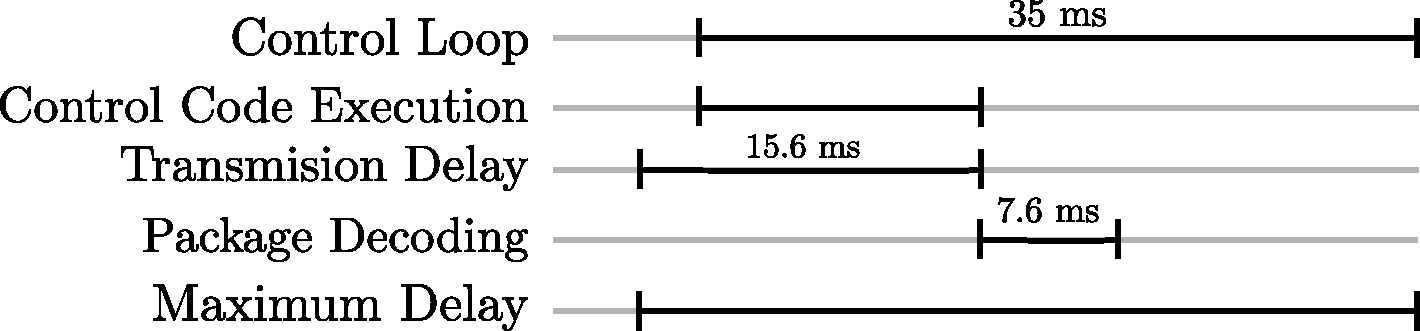
\includegraphics[width=.6\textwidth]{figures/maxDelay.pdf}
	\caption{Delays in the packets transmitted to the microcontroller and maximum delay.}
	\label{fig:delaycontrol}
\end{figure}

After all considerations, the value of the maximum delay which is used in the simulation is \SI{31.46}{ms}.

When considering issues in the network, it is necessary to look into the missed packets. A missed packet can occur if either a new packet is not received between two control loops, making second control loop use old data, or a received packet is corrupted.

This issue can be included in the simulation by utilizing TrueTime. Here the missed packets can be simulated as a constant probability. To get estimate it, tests are conducted in which 10000 packets are transmitted. The amount of packets received correctly and processed in the microcontroller together with the number of control loops executed, provides an estimate of the probability of missing packets. The data obtained with the tests is shown in more detail in \autoref{sec:NetworkTest}. The probability of missing a packet is found to be 0.

The protocol has been design and the main network issues, the delay and missed packets, have been analyzed. This information is used in the design of the controllers.


